\section{Approach}
\label{sec:approach}
In this section, 
we first introduce the length-controllable summarization (LCS) problem,
then introduce the length-aware attention mechanism (LAAM), 
which attends the existing transformer seq2seq models, 
and finally explain how to create a length-balanced dataset (LBD) for pretraining. 

\subsection{Preliminaries}
In LCS, the model takes the source document 
$\mathbf{x} = (x_{0},x_{1},...,x_{m})$ and the desired length $l$ as input and the summary $\mathbf{y} = (y_{0},y_{1},..., y_{n})$ as output. 
$x_i$ is the $i^{th}$ token of document and
$y_t$ is the $t^{th}$ token of summary.
$x_{m}$ and $y_{n}$ are $eos$ tokens.
The goal is to estimate the conditional probability
$p(\mathbf{y}|\mathbf{x})$:
\begin{equation}
	p(\mathbf{y} | \mathbf{x},l) \!=\! {\prod^T_{t} {p(y_{t} | y_{1}, y_{2},..., y_{t-1}, \mathbf{x},l})}
\end{equation}

 
We take the transformer seq2seq model~\cite{attn17} as our basis.
Suppose that the encoder output is $\mathbf{h}=\left\{h_0,h_1,...,h_m\right\}$,  
$\mathbf{h} \in \mathbb{R}^{m \times d}$,
and the output of the decoder's masked self-attention sub-layer 
is $\mathbf{z}=\left\{z_0,z_1,...,z_n\right\}$,
$\mathbf{z} \in \mathbb{R}^{n \times d}$.
The normal cross attention is calculated as:
\begin{equation}
	\mathbf{A}=\softmax(\textbf{z} \cdot \textbf{h}^T)
\end{equation}
where $\mathbf{A} \in R^{n\times m}$ is an attention matrix.
$A_{t}=\left\{a_{t,0}, a_{t,1},...,a_{t,m}\right\}$ shows the attention scores of $y_t$. 
$a_{t,i}$ is the attention score between $y_t$ and $x_i$.

\subsection{Length-aware Attention Mechanism}
\label{sec:model} 
In the transformer seq2seq model, the cross attention of
an output token $y_t$ is likely to \textit{summarize}
those tokens with high attention scores in the input (source document).
By formulating the cross attention as a function of
the desired length $l$, we can manipulate the input
information selection according to $l$. 
This is the intuition behind LAAM,
which is illustrated in \figref{fig:model_main}.
 
\begin{figure}[th]
	\centering
	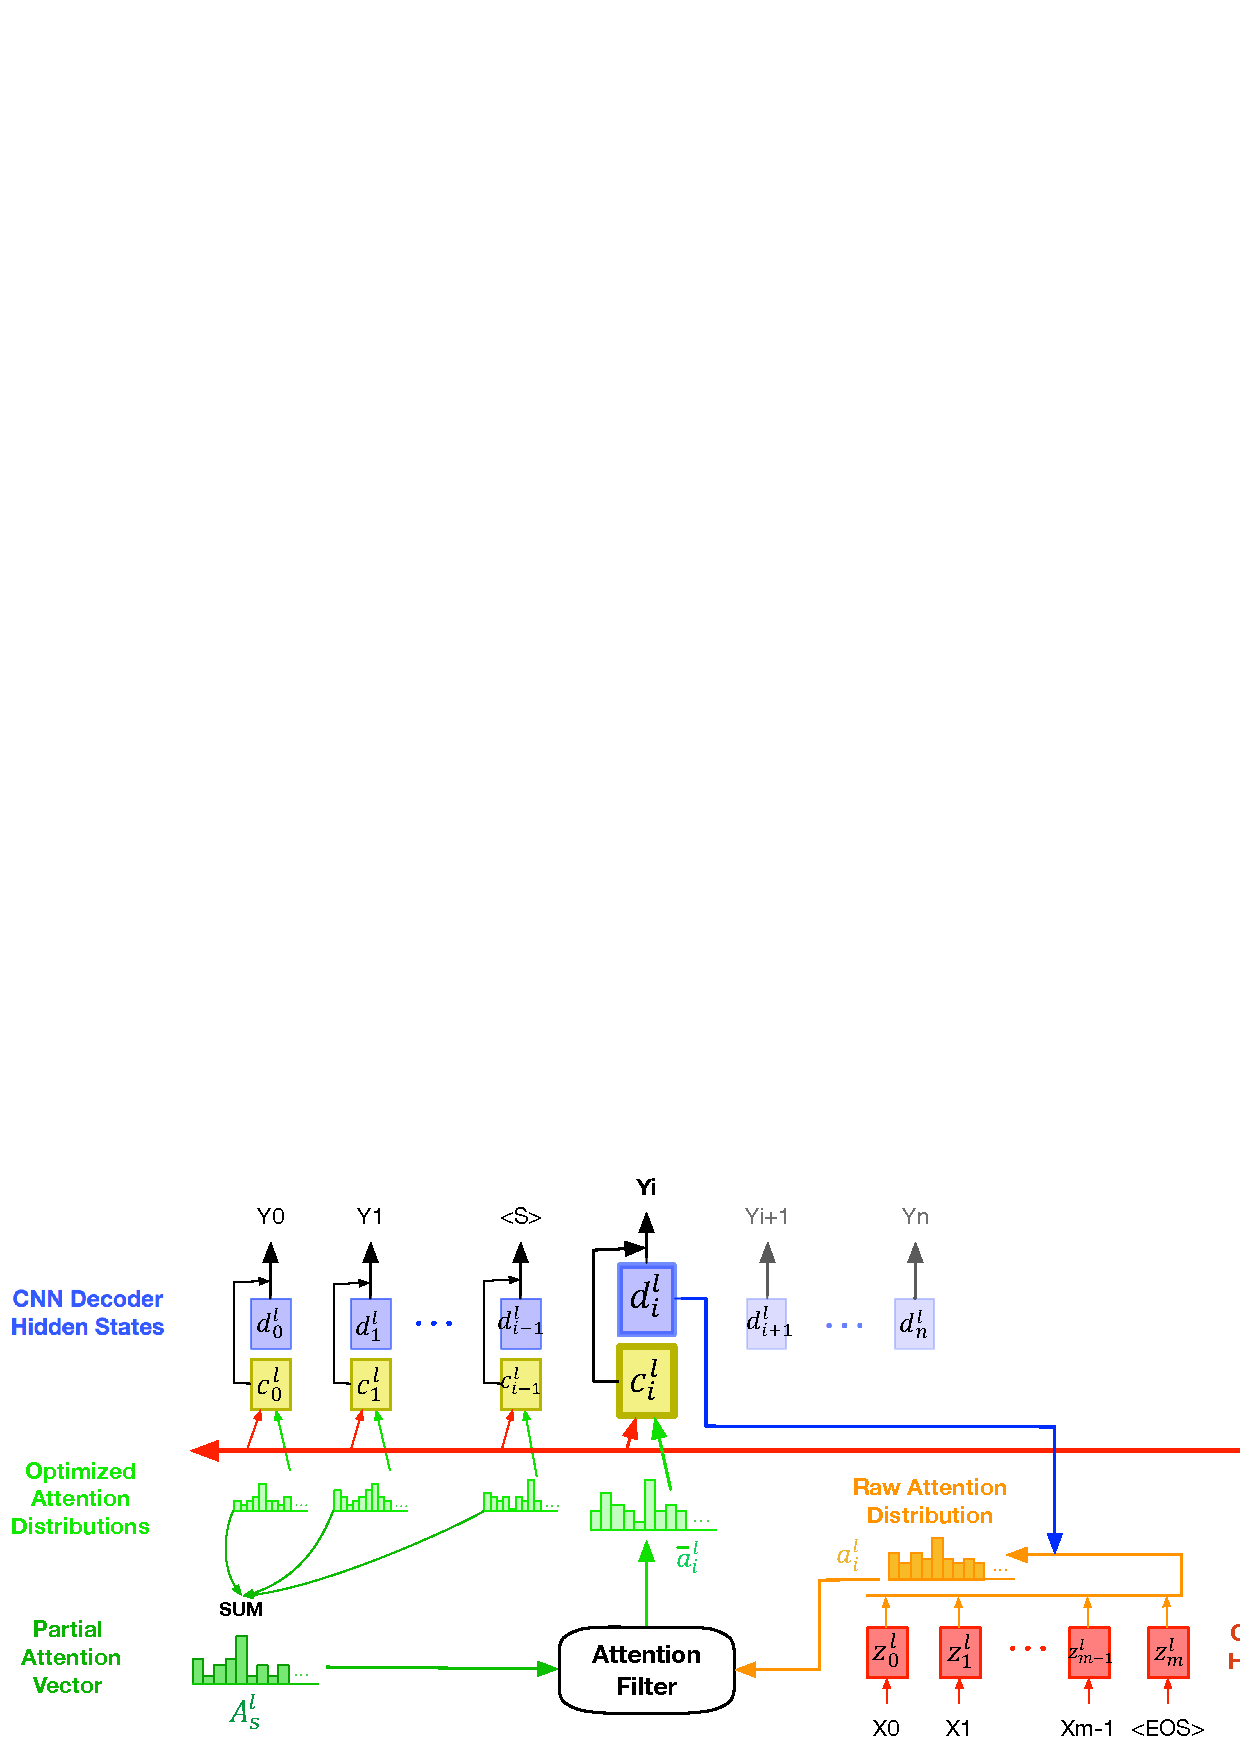
\includegraphics[width=1.0\linewidth]{model.pdf}
	\caption{Overview of LAAM on Transformer Seq2seq. The bold values are boosted attention scores. The shadow boxes denote the attention scores of $eos$.
	}
	\label{fig:model_main}
\end{figure}

LAAM is made up of two parts: {\em attention for input selection} 
($Attn_{is}$) and 
{\em attention for $eos$ token} ($Attn_{eos}$), each optimized for
\textit{information selection} and \textit{length control},
the two objectives in LCS.

$\bm{Attn_{is}}$. At decoding,
given the initial desired length $l$,  $l+1$ is the number of tokens in the output with $eos$, the remaining length budget ($l_t$)
decreases as more tokens are generated. Specifically, at step $t$,
\begin{align}
        l_t &=		
		\begin{cases}			
			l+1-t, &\mbox{$0\leq t \leq l$}\\			
			1, &\mbox{otherwise}			
		\end{cases}		
%	\\
%	   L &=l+1
\end{align}

Intuitively, at each decoding step, 
the decoder should plan its output $y_t$ given the remaining number $l_t$ of 
tokens it will generate.
Our key idea is to increase the attention scores of the top $l_t$ tokens 
with the highest attention scores in $A_t$,
which gives a boost to the chance of these tokens 
to be selected and summarized.
The interesting effect of this is that i) the longer $l$, the more source 
information will be selected for summarization; and ii) as the decoder generates more tokens,the number of tokens to be mainly attended in input decreases.  
We use one-hot vector $\mathbf{p}=\left\{p_0,p_1,...,p_m\right\}$ to 
label the indices of the top $l_t$ tokens with the highest attention scores 
in $A_t$ as $1$ and others as $0$, and then 
the length-aware attention score is computed as:

\begin{align}
	a'_{t,i}=w_{t,i} \times a_{t,i} \\
	w_{t,i}=
		\begin{cases}			
	 		1, &\mbox{$p_i=0$}\\	\label{eq:w}		
	 		l_t, &\mbox{$p_i=1$}			
	 	\end{cases}	
\end{align}

where $w_{t,i}$ is the {\em weight for boosting the attention} between $x_i$ and $y_t$.
According to \eqnref{eq:w},  
the weight for cross attention decreases as the remaining length decreases,
resulting in a decrease in the gap between the enhanced tokens and other tokens. 
This makes the model evenly attend to tokens related to the enhanced tokens and output general words to end the decoding.
The model can learn to select information to be summarized by desired length.


$\bm{Attn_{eos}}$.  At each decoding step $t$, to enhance the ability of model to generate $eos$ at the desired length,
we modify the attention score between $y_t$ and $eos$ in source document $x_m$ as follows:

\begin{equation}
 	a'_{t,m}=(l+1-l_t) \times a_{t,m} \\
\end{equation}
The length-aware attention of $eos$ increases step by step, 
which demonstrates the probability of stopping decoding will increase
as the length of the output close to the desired length.

Finally, we re-normalize the modified attention scores 
$A'_t=\left\{a'_{t,0}, a'_{t,1},...,a'_{t,m}\right\}$ to get the context vector $\mathbf{c_t}$ and compute the probability distribution of 
predicted tokens via:
\begin{align}
	p(y_t|y_{i<t},\mathbf{x},l) &=\softmax(W \mathbf{c}_{t-1}+b) \\
	\mathbf{c_t} &=\sum_{0}^{m} \tilde{a}_{t,i} h_i \\
	\tilde{a}_{t,i} &= \frac{a'_{t,i}}{\sum_{i=0}^{m}a'_{t,i}}
\end{align}
where $W$ and $b$ are trainable parameters.


\subsection{LBD Creation for Pretraining LAAM}
\label{sec:lbd}
Since the summary lengths of a training dataset may be highly concentrated in a small range (see \tabref{tab:lendis}), 
neural-based abstractive summarization models 
tend to select source information according to the summary lengths they have seen in training data and generate summaries with similar lengths.
In order to make the model learn to select proper information according to different desired lengths,
we propose a heuristics to create a length-balanced dataset (LBD) by extracting summaries with various lengths from each document in original dataset and makeing lengths of these extractive summaries evenly distributed in different ranges. 

Given an abstractive summarization dataset $D$, which consists of
a training set $T$ and a validation set $V$, we create the training
set $T'$ and validation set $V'$ of LBD. 
To create $T'$, 
we set the discrete bins $B=\left\{b_1, b_2,...,b_k\right\}$ to represent the ranges of summary length of $T'$. 
$k$ is the number of the bins. 
For example, $B=\left\{(0,10],(10,20],...\right\}$ and $b_0=(0,10]$. 
For each document $src$ and its reference summary $ref$ in $T$,
we produce length-controllable pairs (LCPs) consisting of $src$ and its 
extractive summaries in various length ranges.
Let $e$ be the extractive summary of length $b \in B$. 
We apply a greedy approach,
where we add one sentence at a time incrementally to the $e$, 
until the length of $e$ is within the proper range of $b$ and has the highest 
ROUGE-1 (R-1) recall with respect to $ref$.
Generally, the more training data, the greater the impact on the model.
To make $T'$ effective,
the number of samples in $T'$ should be close to $|T|$.
$S(b)$ is the subset of $T'$, including LCPs with extracted summaries with 
length in $b$. 
We add top $\lceil |T|/k \rceil$ extractive summaries (length $\in b$) 
with the highest R-1 recall and their source documents to $S(b)$,
which makes the summaries equally distributed in the bins or length ranges.
The details are in \algoref{alg:data}. 


\begin{algorithm}[th!]
	\caption{Creating Training Set of LBD}
	\label{alg:data}
	\scriptsize
	\textbf{Input}: the training set $T$ \\
	\textbf{Output}:  the training set $T'$ \\
	\begin{algorithmic}[1] %[1] enables line numbers
		\STATE $rec()$ computes the R-1 recall score between two texts.
		\STATE $len()$ computes the length of token sequence.
		\FOR {\textbf{each} training pair ($src$, $ref$) $\in T$}
		\STATE $src=\left\{s_0, s_1,...\right\}$, where $s_t$ is the $t^{th}$ sentence in $src$.
		\FOR {$i=0 \rightarrow k$}
		\STATE $min$ and $max$ denote minimum and maximum length of length range $b_i$, respectively.
		\STATE $e_i \leftarrow \emptyset$
		\WHILE{$S=\left\{s|s \in src \cap len(e_i \cup s) \leq max \right\}$}
	    \STATE Select the $s_{sel}$ with best $rec(e_i\cup s_{sel}, ref)$ from $S$.
		\IF{$rec(e_i\cup s_{sel}, ref) \textgreater rec(e_i, ref)$}
		\STATE $e_i \leftarrow s_{sel}$; $src \leftarrow src-s_{sel}$
		\ELSE 
		\STATE break
		\ENDIF
		\ENDWHILE
		\IF{$len(e_i) \textgreater min$}
		\STATE Add $(src, e_i, rec(e_i,ref))$ to $S(b_i)$.
		\ENDIF
		\ENDFOR
		\ENDFOR
		\STATE $S(b_i) \leftarrow$ top $\lceil |T|/k \rceil$ samples from $S(b_i)$ sorted by $rec(e_i,ref)$
		\STATE $T' \leftarrow S(b_1) \cup S(b_2)\cup \cdots \cup S(b_k)$
		\RETURN $T'$
	\end{algorithmic}
\end{algorithm}


For $V'$, we create an extractive reference summary by selecting one sentence at a time 
until we get a subset of sentences from $src$ that maximizes the R-1 F1 
with respect to $ref$. 
Given an original source document and reference summary pair, 
R-1 recall computes the similarity between extracted sentences and reference without considering the length of extracted sentences.
This meets our requirements for creating $T'$, that is, we can extract multiple summaries within different length ranges for one document.
To evaluate the model at training,
each document in $V'$ only needs one extractive summary.
R-1 F1 considers the difference between the lengths of compared summaries, 
which can select an extractive summary most similar to the reference in length and content.


In this paper, we first pretrain LAAM on LBD for the ability to select information from source document to be summarized according to length constraint.
Then we fine-tune the pretrained LAAM ({\bf PtLAAM}) on original dataset.
At this stage, armed with the ability to select information from source document, 
the model further learns to paraphrase the selected information into 
abstractive summaries with desired length.

